{%
  \setbeamercolor{background canvas}{bg=black}
  \setbeamercolor{frametitle}{fg=white}
  \begin{frame}
  \frametitle{\bfseries Derivasjon}
  \section{Derivasjon}
  \begin{center}
  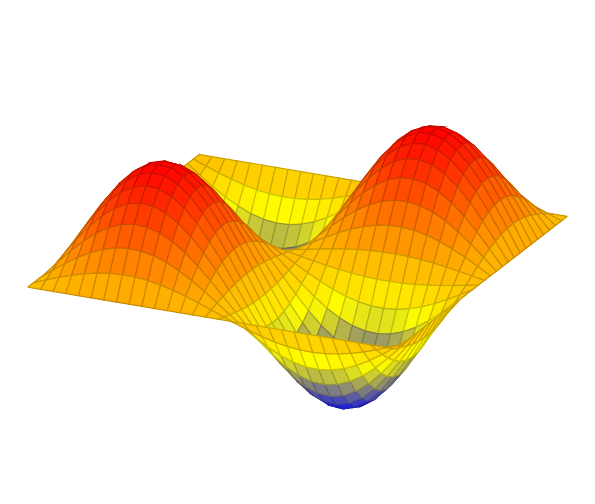
\begin{tikzpicture}
      \begin{axis} [
        xtick = {-50,-60},
        ytick = {-5,-6},
        ztick = {-3,-4},
        ticklabel style = {font = \scriptsize},
        axis line style={draw=none},
        tick style={draw=none}
      ]
      \addplot3 [surf, domain=0:360, samples=30] 
        { sin(x)*sin(y) };
      \end{axis}
    \end{tikzpicture}
    \visible<2>{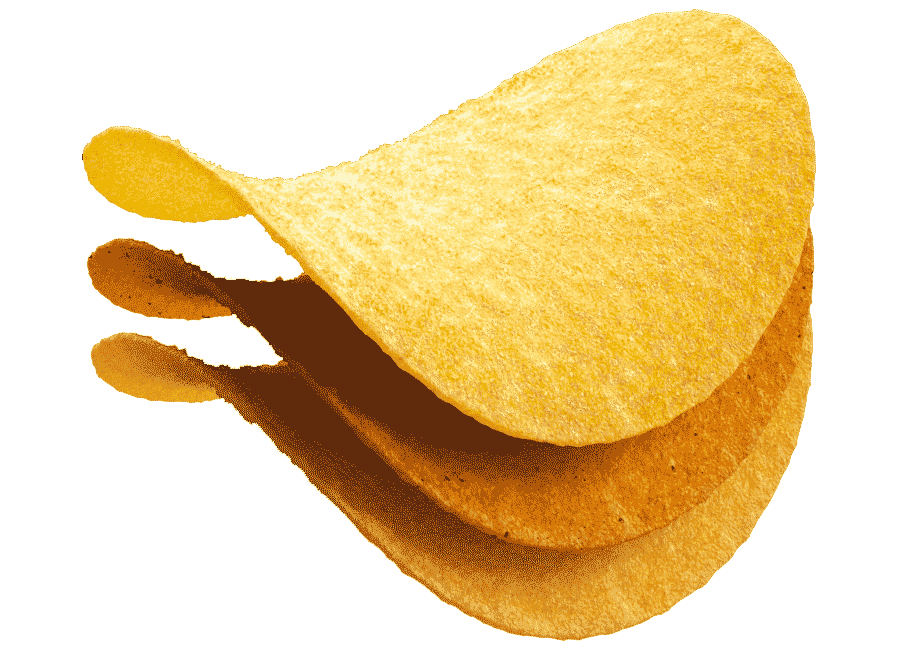
\includegraphics[width=0.4\textwidth]{../img/pringles.png}}
   \end{center}
  \end{frame}%
}

%%% Local Variables:
%%% mode: latex
%%% TeX-master: "main"
%%% End:
